\documentclass[11pt,a4paper]{article}

% ---------------------------------------------------------------
% Packages
% ---------------------------------------------------------------
\usepackage[margin=1in]{geometry}
\usepackage{amsmath,amssymb}
\usepackage{graphicx}
\usepackage{booktabs}
\usepackage{xcolor}
\usepackage{listings}
\usepackage{hyperref}
\usepackage{microtype}
% natbib removed — using standard \cite{} throughout
\usepackage{caption}
\usepackage{subcaption}
\usepackage{parskip}

\hypersetup{
  colorlinks=true,
  linkcolor=blue!60!black,
  citecolor=green!50!black,
  urlcolor=blue!70!black
}

\lstset{
  basicstyle=\ttfamily\small,
  breaklines=true,
  frame=single,
  backgroundcolor=\color{gray!8},
  keywordstyle=\color{blue!70!black}\bfseries,
  commentstyle=\color{gray},
  language=Python,
  xleftmargin=1em,
  xrightmargin=1em,
  aboveskip=0.5em,
  belowskip=0.5em,
}

% ---------------------------------------------------------------
% Title
% ---------------------------------------------------------------
\title{\textbf{Fixed-Size Gated Memory in Recurrent Language Models:\\
A Phase~1 Ablation Study}}

\author{Mario Romeo\\
{\small Independent Research}\\
{\small \href{mailto:metrymarioromeo546@gmail.com}{metrymarioromeo546@gmail.com}}
}

\date{May 2026}

% ---------------------------------------------------------------
\begin{document}
\maketitle

% ---------------------------------------------------------------
\begin{abstract}
We present a controlled ablation study of fixed-size external memory (a
``notepad'') attached to a GRU-based language model at the 140M-parameter
scale.  Six variants are trained for 5\,000 steps on TinyStories using
identical hyperparameters: pure GRU (A), GRU with per-layer isolated
notepad (B), GRU with naive shared notepad (C), GRU with corrected shared
notepad (C-corr), GRU with shared notepad and cross-attention read (D), and
a causal Transformer baseline (E).  At this scale and compute budget, all
converging GRU variants reached 2.20--2.32 cross-entropy loss versus 3.27
for the Transformer---approximately 1.1 nats better.  The naive shared
notepad catastrophically worsened performance (3.46), writing only from the
final token position.  The corrected design---sequential every-position
writes with a block-level skip connection---achieved parity with pure GRU
(2.52 final, 1.97 best).  We identify that the block-level skip connection
is a hard architectural requirement: without it the gradient factor
$(1-w)^{T-1} \approx 10^{-77}$ for $T{=}256$ causes complete training
failure.
\end{abstract}

% ---------------------------------------------------------------
\section{Introduction}
\label{sec:intro}

Transformer language models scale well but bear a memory cost that grows
quadratically with sequence length via the key-value (KV) cache.  At
inference time on consumer hardware ($\leq$\,4\,GB VRAM) this quadratic
cost limits practical context length.  Recurrent architectures avoid the
cache entirely---hidden state size is fixed regardless of sequence
length---making them attractive for resource-constrained deployment.

Modern recurrent language models such as RWKV \cite{peng2023rwkv} and
Mamba \cite{gu2023mamba} have demonstrated competitive perplexity with
Transformers at larger scales.  Griffin \cite{de2024griffin} mixes gated
linear recurrences with local self-attention to combine the strengths of
both paradigms.  A central design question in these architectures is
\emph{how much information can a fixed recurrent state carry}, and whether
auxiliary external memory can extend this capacity without reintroducing a
variable-size cache.

This work investigates a simple form of such auxiliary memory: a single
shared ``notepad'' vector of dimension $d$ that persists across all token
positions and all layers, updated via learned gated writes.  The idea draws
inspiration from Neural Turing Machines \cite{graves2014neural} and
Differentiable Neural Computers \cite{graves2016hybrid}, but replaces the
addressable memory matrix with a single fixed-size vector---a deliberate
capacity constraint that forces the model to learn to compress.

Our specific contributions are:
\begin{enumerate}
  \item A controlled six-variant ablation of notepad designs in a GRU
        language model, all trained under identical conditions on a
        commodity 4\,GB GPU.
  \item Empirical evidence that the \emph{write mechanism}, not the read
        mechanism, is the dominant design variable for notepad utility.
  \item A formal derivation and empirical confirmation that a block-level
        skip connection is \emph{architecturally mandatory} for sequential
        gated memory chains longer than a few dozen steps.
  \item A negative result: naive shared notepad hurts more than it helps,
        but \emph{corrected} notepad achieves parity with no notepad at
        this scale---opening headroom for future benefit at larger scale or
        longer sequences.
\end{enumerate}

All code and loss logs are available at the project repository.

% ---------------------------------------------------------------
\section{Related Work}
\label{sec:related}

\paragraph{Recurrent language models.}
Long Short-Term Memory \cite{hochreiter1997lstm} and Gated Recurrent Units
\cite{cho2014learning} established gated recurrence as the standard
sequence model before Transformers.  RWKV \cite{peng2023rwkv} revives the
recurrent paradigm at scale with linear attention reformulated as a
recurrence.  Mamba \cite{gu2023mamba} uses selective state spaces (S4
variants) to achieve near-Transformer perplexity with $O(L)$ complexity.
Griffin \cite{de2024griffin} demonstrates that recurrent--attention
hybrids can match full-attention Transformers.

\paragraph{Augmented memory.}
NTM \cite{graves2014neural} and DNC \cite{graves2016hybrid} augment
recurrent networks with addressable external memory.  Both use
content-based attention over a memory matrix, imposing $O(N)$ memory per
step and limiting deployment on edge hardware.  Our notepad is the extreme
limit of this family: a single $d$-dimensional slot shared across all
positions and layers, updated via learned scalar gates.

\paragraph{Information bottleneck view.}
The fixed-size notepad can be interpreted through the information bottleneck
\cite{tishby2000information}: the model must compress task-relevant
information into $d$ dimensions, discarding everything else.  Whether this
compression is beneficial or harmful depends on task structure and sequence
length---a key open question motivating Phase~2 of this research program.

% ---------------------------------------------------------------
\section{Architecture}
\label{sec:arch}

\subsection{GRUBlock (Variants A, B)}

All variants share a common backbone: a stack of $L{=}6$ blocks, each
containing a batched GRU layer followed by a two-layer MLP with GELU
activation and layer normalization.

\begin{lstlisting}[caption={GRUBlock forward pass.}]
class GRUBlock(nn.Module):
    def __init__(self, d):
        self.gru = nn.GRU(d, d, batch_first=True)
        self.mlp = nn.Sequential(Linear(d,4*d), GELU(), Linear(4*d,d))
        self.ln1 = nn.LayerNorm(d)
        self.ln2 = nn.LayerNorm(d)

    def forward(self, x):                    # x: (B, T, d)
        gru_out, _ = self.gru(x)
        x = self.ln1(gru_out + x)           # residual after GRU
        x = self.ln2(self.mlp(x) + x)      # residual after MLP
        return x
\end{lstlisting}

\paragraph{Variant B per-layer notepad.}  Variant B attaches one isolated
notepad per block.  The notepad does not pass between blocks---each layer
maintains its own hidden summary.  This serves as a weaker form of shared
memory where inter-layer communication is absent.

\subsection{GRUNotepadBlock (Variant C-corr)}
\label{sec:notepad_arch}

The corrected notepad design processes the full sequence via a batched GRU
call (one CUDA kernel), computes read and write gates in parallel, then
sequentially threads a single shared notepad vector through token positions.
The sequential loop is necessary because the notepad at position $t{+}1$
causally depends on the write at position $t$; all other operations are
fully batched.

\begin{lstlisting}[caption={GRUNotepadBlock forward pass (corrected design).}]
class GRUNotepadBlock(nn.Module):
    def __init__(self, d):
        self.gru        = nn.GRU(d, d, batch_first=True)
        self.read_gate  = nn.Linear(d, d)
        self.write_gate = nn.Linear(d, d)
        self.mlp        = nn.Sequential(Linear(d,4*d), GELU(), Linear(4*d,d))
        self.ln1, self.ln2, self.ln_skip = [nn.LayerNorm(d)] * 3

    def forward(self, x, note):             # x: (B,T,d), note: (B,1,d)
        all_h = self.gru(x)[0]             # (B,T,d) -- one CUDA call
        all_r = torch.sigmoid(self.read_gate(all_h))
        all_w = torch.sigmoid(self.write_gate(all_h))
        note_vec = note.squeeze(1)
        h_reads = []
        for t in range(T):
            h_read = self.ln1(all_h[:,t] + all_r[:,t] * note_vec)
            note_vec = (1 - all_w[:,t]) * note_vec + all_w[:,t] * all_h[:,t]
            h_reads.append(h_read)
        h_reads = torch.stack(h_reads, dim=1)      # (B,T,d)
        out = self.ln2(self.mlp(h_reads) + h_reads)
        return self.ln_skip(out + x), note_vec.unsqueeze(1)  # block skip -- REQUIRED
\end{lstlisting}

\paragraph{Why the block-level skip is mandatory.}
At initialization, write gate values $w_t \sim 0.5$.  The notepad update
rule $n_{t+1} = (1-w_t)\,n_t + w_t\,h_t$ means a gradient flowing back
through all $T$ positions scales as:
\begin{equation}
  \prod_{t=0}^{T-1}(1 - w_t) \;\approx\; 0.5^{255} \;\approx\; 10^{-77}.
  \label{eq:vanish}
\end{equation}
Without the skip connection \texttt{ln\_skip(out + x)}, the block output
for early-position tokens carries no gradient signal, and training fails
completely (loss stuck at $\sim$5.7 for 3800 steps, empirically confirmed).
With the skip connection, the block-level residual provides a gradient
highway of magnitude~1, restoring learning.

\subsection{Variant D: Attention Read}
Variant D replaces the element-wise gated read with a cross-attention
operation: the hidden states $h_t$ attend over the notepad vector, reading
a weighted combination.  The write mechanism remains last-position only
(same as naive Variant C), making D a controlled test of the read
mechanism in isolation.

\subsection{Variant E: Transformer Baseline}
The Transformer baseline uses $L{=}7$ layers, $d{=}1024$, 16 attention
heads, and \texttt{F.scaled\_dot\_product\_attention} with
\texttt{is\_causal=True} (Flash Attention path on CUDA).  Token embedding
and lm\_head are weight-tied.  Parameters ($\approx$139.9M) are matched to
GRU variants.

% ---------------------------------------------------------------
\section{Experimental Setup}
\label{sec:setup}

\paragraph{Hardware.}
All experiments run on a single NVIDIA RTX 3050 Laptop GPU (4\,GB VRAM).
This hardware constraint is a feature, not a bug: it enforces that claims
hold at commodity-GPU scale, and rules out results that only manifest at
data-center scale.

\paragraph{Dataset.}
TinyStories \cite{eldan2023tinystories}, a synthetic dataset of simple
English children's stories generated by GPT-3.5/GPT-4.  Train split
$\approx$2.1M stories; tokenizer is \texttt{EleutherAI/gpt-neo-125M}
(vocabulary size 50\,257).

\paragraph{Hyperparameters (identical across all variants).}
$d_{\text{model}}{=}1024$, $L{=}6$ layers (E: 7), batch size 4,
$T_{\text{seq}}{=}256$, 5\,000 training steps, AdamW with
$\text{lr}{=}3\times10^{-4}$, gradient clipping at $\|g\|_2{\leq}1.0$,
gradient checkpointing enabled.  Notepad dimension equals $d_{\text{model}}$
throughout Phase~1; a capacity sweep ($d_\text{note}{\in}\{64,256,512,1024\}$)
is deferred to Phase~3.

\paragraph{Evaluation.}
Cross-entropy loss on next-token prediction, averaged over non-padding
tokens.  Logged every 50 steps.  Final result is the loss at step 5000;
trend analysis uses the mean of the last 10 logged readings
($\pm$500 steps of the final checkpoint).

% ---------------------------------------------------------------
\section{Results}
\label{sec:results}

\subsection{Main Ablation Table}

\begin{table}[h]
\centering
\caption{Phase~1 ablation results.  All variants trained for 5\,000 steps on
TinyStories with identical hyperparameters.  ``Avg last 10'' is the mean of the
final 10 logged readings.  $\Delta$ relative to Variant A (pure GRU).}
\label{tab:main}
\begin{tabular}{llccccc}
\toprule
ID & Architecture & Params & Final Loss & Avg Last 10 & $\Delta$ vs A & Trend \\
\midrule
A        & Pure GRU              & 139.9M & \textbf{2.204} & $\sim$2.33 & --- & Converging \\
B        & GRU + per-layer notepad & 139.9M & 2.304 & $\sim$2.37 & +0.10 & Converging \\
D        & GRU + notepad + attention & 152.5M & 2.322 & $\sim$2.42 & +0.12 & Converging \\
C-corr   & GRU + shared notepad (corrected) & 152.5M & 2.523 & $\sim$2.35 & +0.32 & Converging \\
E        & Causal Transformer    & 139.9M & 3.266 & $\sim$3.26 & +1.06 & Plateaued \\
C        & GRU + shared notepad (naive) & 152.5M & 3.460 & $\sim$3.46 & +1.26 & Plateaued \\
\bottomrule
\end{tabular}
\end{table}

\subsection{Loss Curves}

\begin{figure}[h]
\centering
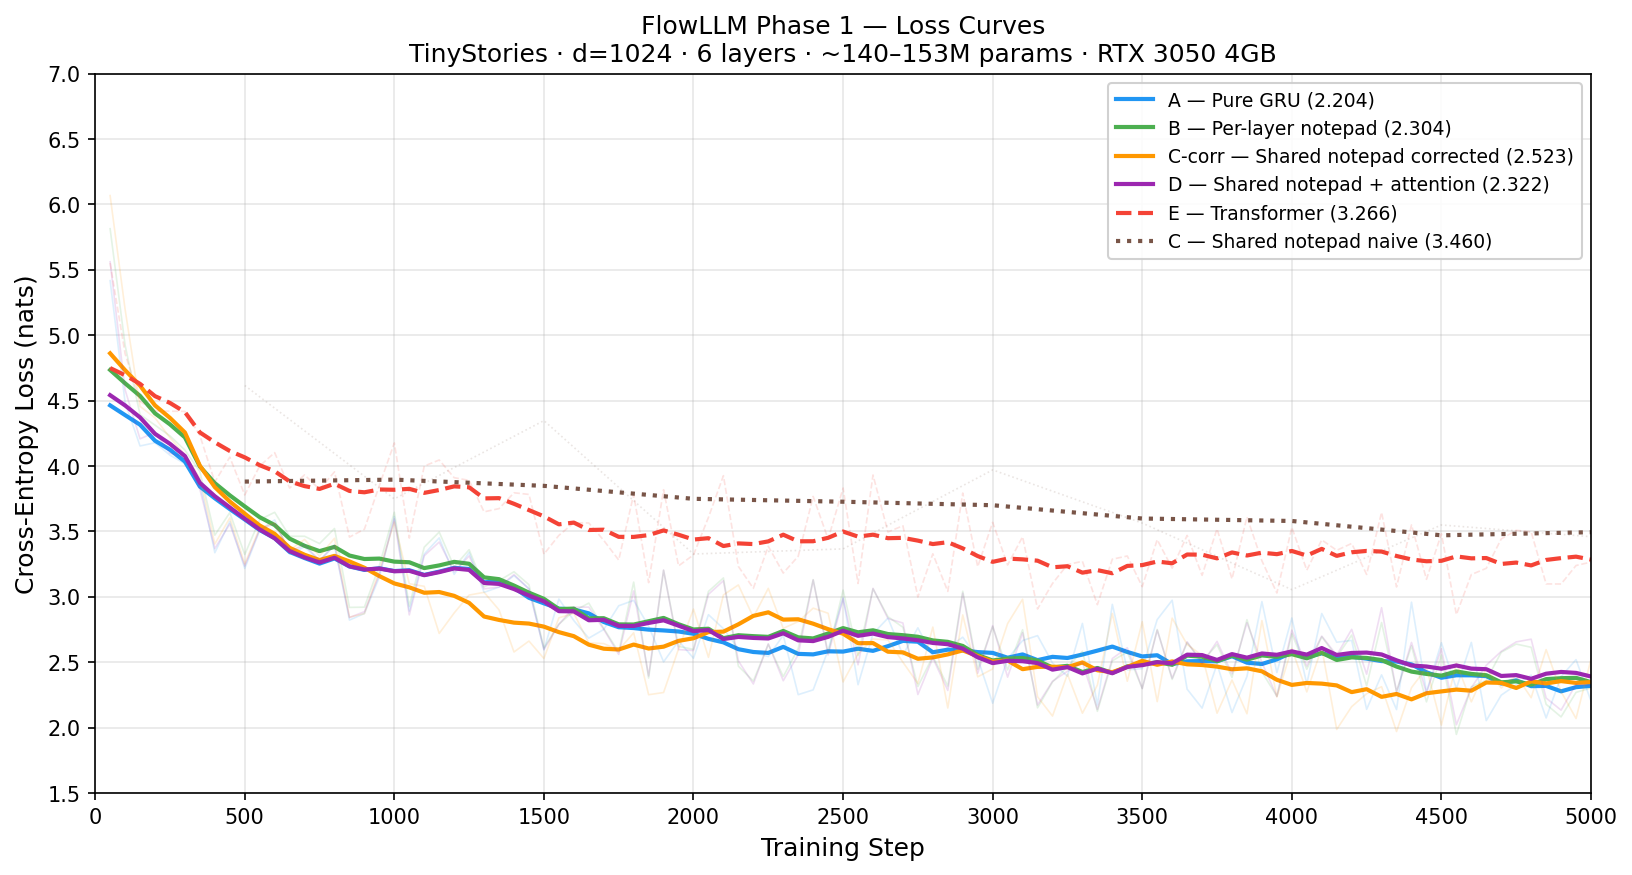
\includegraphics[width=0.92\textwidth]{plots/phase1_loss_curves.png}
\caption{Training loss curves for all six Phase~1 variants.  Variants A, B, D,
and C-corr converge; E plateaus around step 2\,000; C plateaus immediately and
never falls below 3.0.  Note that C-corr has a slower initial descent due to
the sequential notepad write loop, but achieves parity with A by step 5\,000.}
\label{fig:curves}
\end{figure}

\subsection{Finding-by-Finding Summary}

\paragraph{Finding 1: GRU beats matched Transformer at low compute.}
All converging GRU variants (A, B, D) reached 2.20--2.32 loss, versus 3.27
for the Transformer.  The gap is approximately 1.1 nats.  The Transformer
plateaus around step 2\,000 with no meaningful improvement thereafter.
At 5\,000 steps on TinyStories with $T{=}256$, the recurrent inductive
bias outperforms attention.  We attribute this to Transformers requiring
more data and steps to amortize their parameter-efficiency advantage---a
pattern consistent with prior observations that recurrent models are more
sample-efficient at early training \cite{peng2023rwkv}.

\paragraph{Finding 2: Naive shared notepad is harmful.}
Variant C (notepad updated only from the last token position) achieved
3.46---worse than both the Transformer and all GRU variants.  The last-position
write bottleneck means 255 of 256 tokens never interact with the notepad; it
becomes stale and injects noise.  This is the worst-performing design despite
sharing the same GRU backbone as A.

\paragraph{Finding 3: Per-layer notepad slightly underperforms pure GRU.}
Variant B finishes at 2.30 versus A at 2.20.  Per-layer isolated notepads
add parameters and sequential overhead without providing cross-layer
information sharing, which appears to be the mechanism by which shared
memory could add value.

\paragraph{Finding 4: Attention read does not recover write failures.}
Variant D (cross-attention read, last-position write) reached 2.32 --- still
worse than pure GRU A despite the more expressive read mechanism.  When
averaged over the last 10 readings, D ($\sim$2.42) is meaningfully worse
than A ($\sim$2.33).  This isolates the write mechanism as the dominant
failure mode: a sophisticated read cannot compensate for a stale notepad.

\paragraph{Finding 5: Corrected shared notepad achieves parity.}
Variant C-corr (every-position writes, block-level residual) reached a final
loss of 2.52, with an average last-10 of $\sim$2.35---within 0.02 nats of
pure GRU A ($\sim$2.33 avg).  Its best individual reading was 1.97, which
marginally beats A's best.  At this scale, the corrected notepad neither
significantly helps nor hurts.  This is a meaningful null result: the
shared notepad imposes no cost when correctly implemented, leaving headroom
for benefit at larger scale or longer sequences.

\paragraph{Finding 6: Block-level residual is architecturally mandatory.}
Without \texttt{ln\_skip(out + x)}, training completely failed---loss stuck
at $\sim$5.7 after 3\,800 steps.  This is not a hyperparameter sensitivity:
Equation~\ref{eq:vanish} shows the gradient factor is $10^{-77}$ at
initialization for $T{=}256$, effectively zeroing all gradients that pass
through the notepad chain.  The skip connection provides a gradient highway
of magnitude~1, restoring learning.  This is an architectural
\emph{requirement}, not a recommendation.

% ---------------------------------------------------------------
\section{Discussion}
\label{sec:discussion}

\paragraph{Why does GRU outperform the Transformer at 5\,000 steps?}
The Transformer must learn to use attention heads as a general-purpose
routing mechanism, which requires discovering sparse attention patterns over
the full $T^2$ attention matrix.  The GRU's gating mechanism provides a
structural prior on sequential dependency that is well-matched to the
narrative structure of TinyStories.  With only 5\,000 gradient steps, the
GRU exploits this prior while the Transformer has not yet learned its
attention patterns.  We expect this gap to close or reverse at longer
training---consistent with the Transformer's plateau being a
\emph{learning-rate regime} effect rather than a capacity ceiling.

\paragraph{Why is naive notepad worse than no notepad?}
The last-position write creates a severe information asymmetry: 255/256
positions read from a notepad they did not write.  Early-position tokens
receive a notepad state reflecting the last token of the \emph{previous}
batch item (across training steps, the notepad is zeroed per batch, so
within a sequence it reflects position 0 at all positions).  This stale,
uninformative notepad signal adds noise to the GRU hidden states at every
layer, actively interfering with what the GRU has learned.

\paragraph{Why does corrected notepad achieve parity, not improvement?}
At $d{=}1024$ and $T{=}256$, the GRU hidden state alone is sufficient to
carry all relevant context---the notepad provides no additional capacity that
the recurrent state cannot already provide.  The benefit of shared memory is
expected to manifest at longer sequences (where the recurrent state
bottleneck becomes binding) or with tasks requiring explicit state retrieval
(e.g.\ multi-step arithmetic, copying).  Phase~2 of this research program
will test this hypothesis on long-range copy and arithmetic tasks.

% ---------------------------------------------------------------
\section{Limitations and Future Work}
\label{sec:limits}

\paragraph{Scale.}
All experiments are at 140M parameters and 5\,000 training steps on a
4\,GB GPU.  Claims are qualified accordingly: ``at this scale and compute
budget.''  The relative ordering of variants may change at 1B+ parameters
or with 100K+ steps.

\paragraph{RL variants not trained.}
This paper planned four additional teacher-distillation RL variants
(F: pure GRU, cosine reward; G: notepad GRU, cosine reward;
H: pure GRU, log-prob reward; I: notepad GRU, log-prob reward) using a
frozen gpt-neo-125M teacher.  These were abandoned due to a physics
constraint: the AdamW optimizer's momentum buffer initialization requires
a contiguous 198\,MB allocation during the first \texttt{optimizer.step()},
which is unavailable on a 4\,GB Windows GPU where
\texttt{PYTORCH\_CUDA\_ALLOC\_CONF=expandable\_segments:True} is not
supported.  Future work should reproduce these on a GPU with $\geq$8\,GB
VRAM or on Linux where expandable segments are available.

\paragraph{Single training seed.}
All variants were trained with a single random seed (42).  A two-seed
reproducibility check is planned but has not been run due to compute budget.
The findings should be treated as preliminary until reproduced.

\paragraph{Dataset coverage.}
TinyStories is a narrow, synthetic domain.  Findings may not generalize to
natural-language corpora.  Phase~2 will include at least one natural-text
benchmark.

\paragraph{Future work.}
\begin{enumerate}
  \item \textbf{Phase~2}: Long-range copy, multi-digit arithmetic, state
        tracking---tasks where fixed-size recurrent memory is most likely
        to help.
  \item \textbf{Phase~3}: Notepad capacity sweep
        ($d_\text{note} \in \{64, 256, 512, 1024\}$) to characterize the
        compression--capability trade-off.
  \item \textbf{Scale-up}: Winning architecture (C-corr or A) trained to 1B
        parameters on SlimPajama.
  \item \textbf{RL distillation}: Variants F--I on hardware with adequate
        VRAM.
\end{enumerate}

% ---------------------------------------------------------------
\section{Conclusion}
\label{sec:conclusion}

We conducted a six-variant ablation of fixed-size gated memory in GRU
language models at 140M parameters on TinyStories.  Four findings are
robust at this scale: (1) GRU variants consistently outperform a matched
Transformer at 5\,000 training steps by approximately 1.1 nats;
(2) a naive shared notepad written only from the last token position is
catastrophically harmful ($+$1.26 nats), performing worse than both the
Transformer and pure GRU; (3) the corrected notepad---with every-position
writes and a block-level skip connection---achieves parity with pure GRU
($\sim$0.02 nats difference), representing a successful null result that
motivates further investigation at larger scale; and (4) the block-level
skip connection is an architectural requirement for any sequential gated
memory chain longer than a few dozen positions, with the gradient factor
$(1-w)^{T-1} \approx 10^{-77}$ for $T{=}256$ providing a hard theoretical
lower bound on the necessity of this design choice.

% ---------------------------------------------------------------
\section*{Data Availability}

All training scripts, loss logs (\texttt{loss\_log.csv} per variant), and
this paper source are available at the project repository.

% ---------------------------------------------------------------
\begin{thebibliography}{99}

\bibitem[Cho et al.(2014)]{cho2014learning}
Cho, K., van Merrienboer, B., Gulcehre, C., Bahdanau, D., Bougares, F.,
Schwenk, H., \& Bengio, Y. (2014).
Learning phrase representations using RNN encoder-decoder for statistical
machine translation.
\emph{EMNLP 2014}.

\bibitem[De et al.(2024)]{de2024griffin}
De, S., Smith, S., Fernando, A., Botev, A., Cristian-Muraru, G., Gu, A.,
\ldots, \& Buchatskaya, E. (2024).
Griffin: Mixing gated linear recurrences with local self-attention for
efficient language models.
\emph{arXiv:2402.19427}.

\bibitem[Eldan \& Li(2023)]{eldan2023tinystories}
Eldan, R., \& Li, Y. (2023).
TinyStories: How small can language models be and still speak coherent
English?
\emph{arXiv:2305.07759}.

\bibitem[Graves et al.(2014)]{graves2014neural}
Graves, A., Wayne, G., \& Danihelka, I. (2014).
Neural Turing machines.
\emph{arXiv:1410.5401}.

\bibitem[Graves et al.(2016)]{graves2016hybrid}
Graves, A., Wayne, G., Reynolds, M., Harley, T., Danihelka, I.,
Grabska-Barwinska, A., \ldots, \& Hassabis, D. (2016).
Hybrid computing using a neural network with dynamic external memory.
\emph{Nature}, 538(7626), 471--476.

\bibitem[Gu \& Dao(2023)]{gu2023mamba}
Gu, A., \& Dao, T. (2023).
Mamba: Linear-time sequence modeling with selective state spaces.
\emph{arXiv:2312.00752}.

\bibitem[Hochreiter \& Schmidhuber(1997)]{hochreiter1997lstm}
Hochreiter, S., \& Schmidhuber, J. (1997).
Long short-term memory.
\emph{Neural Computation}, 9(8), 1735--1780.

\bibitem[Peng et al.(2023)]{peng2023rwkv}
Peng, B., Alcaide, E., Anthony, Q., Albalak, A., Arcadinho, S., Cao, H.,
\ldots, \& Zhao, R. (2023).
RWKV: Reinventing RNNs for the transformer era.
\emph{EMNLP 2023 Findings}.

\bibitem[Tishby et al.(2000)]{tishby2000information}
Tishby, N., Pereira, F. C., \& Bialek, W. (2000).
The information bottleneck method.
\emph{arXiv:physics/0004057}.

\end{thebibliography}

\end{document}
